%% Pattern Recognition submission. Template required by the journal: elsarticle.cls with
%% \documentclass[times, review, 10pt]{elsarticle} (review = single column, 1.5 line spacing).
%% Page layout as requested by the editorial office: Letter paper, margins 4.3/4.8/4.3/4.8 cm (T/R/B/L),
%% Times, 10 pt text, 8 pt captions/footnotes/authors, numbered pages, page number 2.6 cm from the bottom.
%% Every number comes from tables/macros.tex (generated by code/experiments/aggregate.py).
\documentclass[times, review, 10pt]{elsarticle}

\usepackage[letterpaper, top=4.3cm, right=4.8cm, bottom=4.3cm, left=4.8cm, footskip=1.7cm]{geometry}
\usepackage{graphicx}
\usepackage{amsmath,amssymb}
\usepackage{amsthm}
\usepackage{booktabs}
\usepackage{tabularx}
\usepackage{multirow}
\usepackage{algorithm}
\usepackage{algpseudocode}
\usepackage[shortlabels]{enumitem}
\usepackage{pifont}
\usepackage{xcolor}
\usepackage[font=footnotesize,labelfont=bf,labelsep=period]{caption}
\usepackage[colorlinks=true,linkcolor=black,citecolor=black,urlcolor=black]{hyperref}
\usepackage[section]{placeins}  % floats stay within their section, near their first mention
\usepackage{xr-hyper}
\externaldocument[S-]{supplement_pr}

\newcommand{\cmark}{\ding{51}}
\newcommand{\xmark}{\ding{55}}
\newcommand{\botrule}{\bottomrule}
\input{tables/macros.tex}
\makeatletter\newcommand\tabinput[1]{\@@input #1 }\makeatother

\newtheorem{proposition}{Proposition}
\newtheorem{assumption}{Assumption}
\renewcommand{\theassumption}{A\arabic{assumption}}

\journal{Pattern Recognition}
\date{}
\makeatletter  % first page: plain centred page number instead of the too-wide preprint footer
\def\ps@pprintTitle{\let\@oddhead\@empty\let\@evenhead\@empty\def\@oddfoot{\reset@font\hfil\thepage\hfil}\let\@evenfoot\@oddfoot}
\makeatother
\renewcommand{\topfraction}{0.9}
\renewcommand{\bottomfraction}{0.8}
\renewcommand{\textfraction}{0.07}
\renewcommand{\floatpagefraction}{0.75}
\setcounter{topnumber}{3}
\setcounter{totalnumber}{4}

\begin{document}

\begin{frontmatter}

\title{Duplicate Rows Inflate Conformal Coverage: A Simple Check and Fix for New Cases}

\author[vit]{{\footnotesize P. N. Bhargav Teja}}
\author[vit]{{\footnotesize Rajay Vedaraj I. S.}\corref{cor1}}
\ead{rajay@vit.ac.in}
\cortext[cor1]{Corresponding author.}
\affiliation[vit]{organization={Vellore Institute of Technology},
            country={India}}

\begin{abstract}
A software quality team that attaches 90\% prediction sets to a defect classifier usually checks the promise on a random test split. In tabular data with repeated rows, this check is misleading: many test rows have an exact copy in the training data, so the check averages over easy repeats and the genuinely new cases that matter after deployment. We propose a check--fix--report routine. The check predicts from the data alone, before any model is trained, how far coverage of new cases can fall. The fix calibrates seen and new cases separately. The report states new-case coverage next to the usual figure. We tested the routine with random forests, LightGBM and linear models on \NCsNFlagTotal{} application data sets (software defects, network intrusion, phishing), \NNTotal{} benchmark data sets, controlled copy experiments, and \NScpN{} fresh data sets analysed under plans fixed in advance. On NASA mc1, random-forest sets reported \NCsMcOneReported{}\% coverage but covered \NCsMcOneNew{}\% of new modules, and \NCsMcOneFixed{}\% with the fix. On the fresh data, the check flagged all \NScpPos{} data sets whose new cases fell more than 2 percentage points short, and with the fix new-case coverage never fell more than \NWTwoWorstFixAbs{} points below the target. The check is a warning and a limit rather than a forecast: on the first fresh collection it did not rank data sets by the size of their shortfall. The routine is available as an open-source tool.

\end{abstract}

\begin{keyword}
Conformal prediction \sep Uncertainty quantification \sep Duplicate records \sep Data leakage \sep Software defect prediction \sep Tabular data
\end{keyword}

\end{frontmatter}

\section{Introduction}\label{sec:intro}

Suppose a software quality team uses a classifier to flag modules that are likely to contain defects. A yes/no answer is not enough to plan code reviews, so the team wraps the classifier in conformal prediction. For each module it then gets a small set of labels that is promised to contain the true label 90\% of the time \citep{vovk2022}. Before trusting the promise, the team checks it in the usual way: it splits its historical data at random into training, calibration and test parts and counts how often the sets were right. The answer is close to 90\%, and the system goes into use.

The team may not have noticed that its data contain many repeated rows. In the public NASA defect data, large shares of modules have exactly the same metric values as other modules, as \citet{gray2011} first reported and \citet{shepperd2013} confirmed in a wider audit. Repeats like these are common in tabular data: the same network connection logged thousands of times, the same customer profile entered twice, identical laboratory readings. A random split then places copies of many test rows in the training part. The model has, in effect, seen those answers, so its sets are almost always right for them. The 90\% the team measured is an average over these easy repeats and the cases that are really new. New modules, which are what the team will face after deployment, may be covered much less often.

This is not a hypothetical concern. On the NASA mc1 data, a random forest's 90\% sets were right for \NCsMcOneReported{}\% of test modules but only for \NCsMcOneNew{}\% of new ones, and \NToolStdEmpty{} of the new modules received an empty set (Sect.~\ref{sec:case}). Repeated rows and other leakage are known to inflate accuracy: \citet{kaufman2012} and \citet{kapoor2023} describe leakage in general, and two recent preprints measure the effect of repeated rows on tabular benchmarks: on accuracy and model ranking \citep{li2026}, and on its growth with model flexibility \citep{roth2026}. Their effect on uncertainty estimates has received little attention, although here a stated guarantee, not only an estimate, is what fails without warning.

\subsection*{Motivation and contributions}

We want a procedure that a practitioner can apply before training anything, that repairs the problem when it exists, and that costs nothing when it does not. This paper makes four contributions.

\begin{enumerate}
\item \textbf{A label-aware check that needs no model} (Sect.~\ref{sec:check}). Two closed-form quantities, the expected share of seen test rows and the share whose training copies carry the same label, give a predicted worst-case shortfall for new cases. The first quantity is elementary. The closed form of the second and the resulting shortfall formula are, to our knowledge, new.
\item \textbf{A fix and a reporting rule} (Sect.~\ref{sec:fix}). Calibrating seen and new cases separately is standard Mondrian conformal prediction \citep{vovk2022}. We show that it is the right choice of groups here, and we add a safety margin for small calibration sets and a distance-based variant for near-copies.
\item \textbf{An evaluation under plans fixed in advance} (Sects.~\ref{sec:framework}--\ref{sec:results}). The evaluation covers \NCsNFlagTotal{} application data sets in three domains, \NNTotal{} benchmark data sets, controlled experiments with exact and noisy copies, and two fresh collections of \NPrN{} and \NWTwoN{} data sets analysed under time-stamped plans. Negative results are reported with the positive ones.
\item \textbf{An open-source tool}, \emph{covercheck} (Sect.~\ref{sec:tool}). It runs the routine from the command line or from Python and writes a one-page report. It reproduced the pipeline's results on \NTvN{} data files downloaded fresh from their source.
\end{enumerate}

\subsection*{Organization}

Section~\ref{sec:literature} reviews related work. Section~\ref{sec:prelim} introduces notation and assumptions. Section~\ref{sec:method} presents the routine and its theory. Section~\ref{sec:framework} describes the data, metrics, baselines and hypotheses. Section~\ref{sec:results} reports the results, including ablations, cost, a case study and a discussion with limitations. Section~\ref{sec:conclusion} concludes. Proofs, per-data-set tables and the full deviation log are in the Supplementary Material.

\section{Literature review}\label{sec:literature}

\subsection{Conformal prediction and what it guarantees}
Split (inductive) conformal prediction turns any fitted model into prediction sets or intervals with a finite-sample coverage guarantee, provided calibration and test data are exchangeable. \citet{papadopoulos2002} introduced the inductive form for regression, \citet{lei2018} analysed its distribution-free guarantees, and \citet{vovk2022} give the full theory, including the Mondrian variant used here. \citet{angelopoulos2023} provide an accessible introduction. Several nonconformity scores are standard. \citet{sadinle2019} use $1-\hat p_y$ to obtain the smallest sets for classification, \citet{romano2020a} propose adaptive scores whose sets grow with uncertainty, and \citet{romano2019} conformalize quantile regression for intervals. Recent work in this journal continues to refine scores and set construction: rank-based prediction sets for reliable classification \citep{luo2026rank}, and a score function designed for rule-based binary classifiers \citep{narteni2026}. \citet{vovk2025e} recasts conformal prediction in terms of e-values.

The guarantee is \emph{marginal}: it holds on average over test cases. \citet{vovk2012} showed that conditional validity can only be approximated, and \citet{foygelbarber2021} proved that exact coverage for every input is impossible without further assumptions. When test data differ from calibration data, other methods are needed. \citet{tibshirani2019} reweight calibration scores under covariate shift, \citet{barber2023} bound the coverage loss beyond exchangeability, and \citet{hallberg2026} adapt conformal inference online when the data drift. Conformal prediction is increasingly applied: \citet{norinder2014} introduced it to predictive modelling in chemistry, \citet{morger2021} assessed its calibration for toxicological models, and \citet{hernandez2026} study it for drug-response prediction under strong distribution shift.

\subsection{Group-wise and conditional calibration}
Coverage within a fixed set of groups can be obtained by calibrating each group separately, which is Mondrian conformal prediction \citep{vovk2022}. More general schemes calibrate over richer families. \citet{guan2023} localizes the calibration around each test point, \citet{gibbs2025} give guarantees over a class of covariate shifts, and \citet{bastani2022} obtain multivalid coverage over many overlapping groups. Group-wise calibration has been applied to protected groups, to equalize coverage across them \citep{romano2020b}; to classes, to reduce bias in imbalanced problems \citep{lofstrom2015} or at scale by clustering many classes \citep{ding2023}; to difficulty bins in regression \citep{bostrom2020}; to two-level hierarchical groups \citep{dunn2023}; to categories from improved decision trees in conformal predictive systems \citep{zhang2026}; and to spatial regions \citep{seo2026}.
Training-conditional guarantees, which hold with high probability over the calibration draw, go back to \citet{vovk2012}. Locally adaptive scores, such as the residuals normalized by a nearest-neighbour difficulty estimate of \citet{papadopoulos2011}, give tighter intervals in easy regions. All of these are tools that we use. None of these works asks which groups are needed when a data set contains repeated rows, or how to tell in advance whether it matters.

\subsection{Repeated rows, leakage and evaluation}
Information that leaks from evaluation data into training is a well-known source of over-optimism. \citet{kaufman2012} formalized leakage in data mining, and \citet{kapoor2023} documented its effect on the reproducibility of machine-learning-based science. Overlap between training and test data has been found in many domains. \citet{barz2020} found near-duplicates of test images in CIFAR training sets. \citet{lee2022} showed that duplicated text affects language models. \citet{lewis2021} found test questions repeated in training data for question answering. \citet{elangovan2021} quantified memorization in NLP evaluation. \citet{allamanis2019} reported duplicated code inflating results for code models. For tabular data, \citet{gray2011} and \citet{shepperd2013} documented repeated and inconsistent records in the NASA defect data, and \citet{tavallaee2009} the heavy redundancy of KDD Cup'99. \citet{sheridan2013} recommends time-based splits when records arrive over time. Three recent preprints study repeated rows across many tabular data sets. \citet{li2026} shows that random splits inflate accuracy and can change which model looks best. \citet{roth2026} finds that this kind of leakage grows with model flexibility. \citet{deng2026} audits anomaly-detection benchmarks and builds a detector whose false-alarm rate, calibrated with split conformal prediction, does not change when rows are replicated. These studies concern accuracy, ranking or unsupervised false-alarm control, not the coverage of conformal prediction sets for new cases.

\subsection{Benchmarks and tools}
We use the OpenML platform \citep{vanschoren2014} with its benchmark suites OpenML-CC18 \citep{bischl2021} and OpenML-CTR23 \citep{fischer2023}. Two further collections serve as fresh data: the AutoML Benchmark \citep{gijsbers2024} and the tabular benchmark of \citet{grinsztajn2022}. We also use the UCI repository \citep{kelly_uci}. Models are fitted with scikit-learn \citep{pedregosa2011}, random forests \citep{breiman2001} and LightGBM \citep{ke2017}.

\subsection{Motivations}
Table~\ref{tab:related} compares the closest work with ours. The comparison leads to five motivations.
\begin{enumerate}[(i)]
\item Conformal coverage is checked on random splits, but no work examines what that check means when test rows have training copies.
\item The groups that need separate calibration are usually chosen by the analyst, such as classes, protected groups or regions. Here they are implied by the data, through the seen/new split.
\item Practitioners need to know \emph{before} training whether a problem exists. No existing tool predicts the size of the shortfall from the data alone.
\item Studies of duplicates measure accuracy or ranking. They do not propose a repair that keeps the data and gives a guarantee for new cases.
\item Claims about evaluation practice should be tested on data that were not used to develop them, under a plan fixed in advance.
\end{enumerate}

\begin{table}[!htbp]
\caption{The closest prior work compared with this paper. \cmark: the property is a main subject of the work; --: not addressed. Rep.: studies repeated rows; Cov.: gives a conformal coverage guarantee; New: examines coverage for new (unseen) records; Pre.: predicts the risk before training; Fix: proposes a repair; Tab.: tabular data; Tool: provides a usable software tool.}\label{tab:related}
\centering\scriptsize
\setlength{\tabcolsep}{2.5pt}
\begin{tabularx}{\textwidth}{@{}Xccccccc@{}}
\toprule
Work & Rep. & Cov. & New & Pre. & Fix & Tab. & Tool\\
\midrule
Split conformal prediction \citep{lei2018,vovk2022} & -- & \cmark & -- & -- & -- & \cmark & -- \\
Class-conditional CP \citep{lofstrom2015,ding2023} & -- & \cmark & -- & -- & -- & \cmark & -- \\
Conditional guarantees \citep{gibbs2025,bastani2022} & -- & \cmark & -- & -- & -- & \cmark & -- \\
Difficulty Mondrian CP \citep{bostrom2020} & -- & \cmark & -- & -- & -- & \cmark & -- \\
Normalized nearest-neighbour scores \citep{papadopoulos2011} & -- & \cmark & -- & -- & -- & \cmark & -- \\
Spatial Mondrian CP \citep{seo2026} & -- & \cmark & -- & -- & -- & \cmark & -- \\
Leakage in ML science \citep{kaufman2012,kapoor2023} & \cmark & -- & -- & -- & \cmark & \cmark & -- \\
Duplicates in code and text \citep{allamanis2019,lee2022} & \cmark & -- & \cmark & -- & \cmark & -- & -- \\
Defect and intrusion data quality \citep{shepperd2013,tavallaee2009} & \cmark & -- & -- & -- & \cmark & \cmark & -- \\
Duplicates in tabular benchmarks \citep{li2026,roth2026} & \cmark & -- & -- & -- & -- & \cmark & -- \\
Replication-robust anomaly detection \citep{deng2026} & \cmark & \cmark & -- & -- & \cmark & \cmark & -- \\
\midrule
This paper & \cmark & \cmark & \cmark & \cmark & \cmark & \cmark & \cmark \\
\bottomrule
\end{tabularx}
\end{table}

\section{Preliminary concepts}\label{sec:prelim}

\paragraph{Data and splits.} A data set $D=\{(x_i,y_i)\}_{i=1}^{N}$ is split uniformly at random into a training part $T$ with $n_T$ rows, a calibration part $C$ with $n_C$ rows and a test part $E$ (60/20/20 in all our experiments). Rows with exactly the same feature vector form a \emph{record group}; $m_j$ is the size of the group of row $j$. A calibration or test row is \emph{seen} if some training row has the same feature vector, and \emph{new} otherwise. We write $\kappa_T(x)\in\{\mathrm S,\mathrm N\}$ for this label. It depends only on the training features.

\paragraph{Split conformal prediction.} A model fitted on $T$ yields a nonconformity score $s(x,y)$. We use $s=1-\hat p_y(x)$ for classification and $s=|y-\hat y(x)|$ for regression. With target miscoverage $\alpha$ (we use $\alpha=0.1$, a 90\% target), the prediction set is
\begin{equation}
\mathcal C(x)=\{y:\ s(x,y)\le \hat q\},\qquad \hat q=\text{the }\lceil (n_C+1)(1-\alpha)\rceil\text{-th smallest calibration score.}\label{eq:scp}
\end{equation}

\paragraph{Coverage of seen and new cases.} Write $\pi$ for the share of test rows that are seen, $c$ for overall coverage, and $c_{\mathrm S}$ and $c_{\mathrm N}$ for the coverage of seen and new rows. Because a test row is either seen or new,
\begin{equation}
c=\pi c_{\mathrm S}+(1-\pi)c_{\mathrm N},\qquad\text{so}\qquad c_{\mathrm N}=\frac{c-\pi c_{\mathrm S}}{1-\pi}.\label{eq:decomp}
\end{equation}
Split conformal prediction keeps $c$ near $1-\alpha$. New cases are therefore under-covered exactly when seen cases are over-covered. If every seen row is covered ($c_{\mathrm S}=1$), the miss rate on new cases is $\alpha/(1-\pi)$ instead of $\alpha$. With half of the test rows seen, one new case in five is missed while the usual check still reports 90\%.

\paragraph{Assumptions.} The guarantees and predictions below rest on three assumptions, which we test.
\begin{assumption}[Random split]\label{as:split}
$T$, $C$ and $E$ are a uniformly random partition of $D$. Given $T$, the remaining rows are therefore still assigned to $C$ and $E$ at random, and $\kappa_T$ is a fixed function.
\end{assumption}
\begin{assumption}[Memorization]\label{as:mem}
A row whose training copies all carry exactly its label (or target value) receives the lowest possible score.
\end{assumption}
\begin{assumption}[Equal difficulty]\label{as:equal}
All other rows, both new rows and seen rows whose copies disagree on the label, have scores from one common continuous distribution $F$.
\end{assumption}
Assumption~\ref{as:split} is the standard condition for split conformal prediction and holds by construction in our experiments. Assumptions~\ref{as:mem} and~\ref{as:equal} are idealizations used only for the predicted shortfall. Flexible models approach \ref{as:mem}, and regularized models do not. Assumption~\ref{as:equal} fails when repeated rows disagree slightly but are still easy, and when seen rows with conflicting labels are \emph{harder} than new ones. We report both failure modes (Sect.~\ref{sec:res-fresh}).

\section{Proposed methodology}\label{sec:method}

\subsection{Overview}
The routine has three steps (Fig.~\ref{fig:schematic}, Algorithm~\ref{alg:routine}). The \emph{check} uses only the features and labels of the full data set: it predicts how many test rows a random split will place next to a training copy, and how much this can depress coverage for new cases. The \emph{fix} calibrates seen and new rows separately, which restores the promise for new cases whatever the model. The \emph{report} states coverage on new cases next to the usual overall figure. Which parts are standard and which are new is stated with each result.

\begin{figure}[!htbp]
\centering
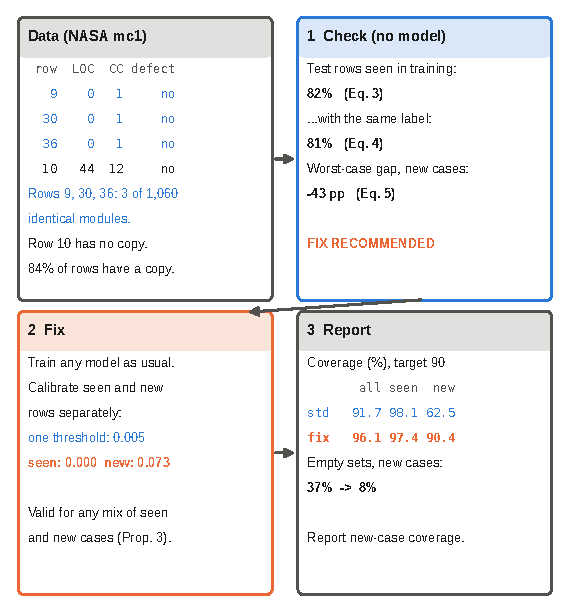
\includegraphics[width=\textwidth]{figures/fig_schematic.pdf}
\caption{The check--fix--report routine, shown with real rows of the NASA mc1 defect data. The check predicts a large shortfall before any model is trained, and the fix restores new-case coverage. The rows shown follow a fixed rule: the first three rows of the largest group of identical modules, and the first row with no copy. All numbers come from the experiment files (random forest, 10 random splits). LOC: lines of code; CC: cyclomatic complexity}\label{fig:schematic}
\end{figure}

\begin{algorithm}[!htbp]
\caption{Check, fix and report conformal coverage for new cases}\label{alg:routine}
\begin{algorithmic}[1]
\Require data $D$, target miscoverage $\alpha$, training share $f$
\Statex \hspace{\algorithmicindent}tolerances $\tau_g=0.02$ and $\tau_\pi=0.10$
\State \textbf{Check} (no model): hash every feature vector; for each row $j$ count its copies $m_j-1$ and the copies with a different label $d_j$
\State compute $\bar\pi$ (Eq.~\ref{eq:exposure}), $\bar\pi_P$ (Eq.~\ref{eq:pure}) and $g^*=-\alpha\bar\pi_P/(1-\bar\pi_P)$ (Eq.~\ref{eq:gstar})
\State \textbf{if} $g^*<-\tau_g$ \textbf{or} $\bar\pi\ge\tau_\pi$ \textbf{then} flag the data set
\State split $D$ at random into $T$, $C$, $E$; fit any model on $T$
\State \textbf{Fix}: label each calibration and test row seen or new by exact match with $T$
\State compute one threshold per group: $\hat q_k=$ the $\lceil (n_k+1)(1-\alpha)\rceil$-th smallest calibration score in group $k$ ($+\infty$ if $n_k<1/\alpha-1$)
\State optionally use the safety-margin rank (Eq.~\ref{eq:pac}) or distance groups instead of seen/new
\State \textbf{Report}: coverage on all, seen and new test rows; for deployment use $\mathcal C(x)=\{y: s(x,y)\le \hat q_{\kappa_T(x)}\}$
\end{algorithmic}
\end{algorithm}

\subsection{Step 1: the check}\label{sec:check}
\paragraph{Exposure.} If a test row belongs to a group of $m_j$ identical rows, and $n_T$ of the other $N-1$ rows go to training, the chance that none of its $m_j-1$ copies lands in training is $\binom{N-m_j}{n_T}/\binom{N-1}{n_T}$. The expected share of seen test rows is therefore
\begin{equation}
\bar\pi=\frac1N\sum_{j=1}^{N}\Big[1-\binom{N-m_j}{n_T}\Big/\binom{N-1}{n_T}\Big].\label{eq:exposure}
\end{equation}
This is elementary combinatorics; \citet{li2026} gives the analogous probability for cross-validation.

\paragraph{Label purity.} Exposure alone can mislead. If repeated rows disagree on the label (identical survey profiles with different outcomes, for example), memorizing them does not help the model. Let $d_j$ be the number of copies of row $j$ whose label (or target value) differs from $y_j$. Row $j$ is \emph{label-pure seen} if at least one copy, but no differently labelled copy, lands in training. Its expected share is
\begin{equation}
\bar\pi_P=\frac1N\sum_{j=1}^{N}\Big[\binom{N-1-d_j}{n_T}-\binom{N-m_j}{n_T}\Big]\Big/\binom{N-1}{n_T}.\label{eq:pure}
\end{equation}

\begin{proposition}[Closed-form label-pure exposure]\label{prop:pure}
Under Assumption~\ref{as:split}, the expected share of test rows that are label-pure seen equals $\bar\pi_P$ in Eq.~(\ref{eq:pure}).
\end{proposition}
The proof is in Sect.~\ref{S-sec:proofs} of the Supplementary Material. On five data sets, the closed form agreed with an average over 30 random splits to within \NPureCfMaxdiff{}.

\paragraph{Predicted shortfall.} Under Assumptions~\ref{as:mem} and~\ref{as:equal}, calibration scores come from a mixture with mass $\pi_P$ at zero and mass $1-\pi_P$ spread by $F$.

\begin{proposition}[Memorization limit]\label{prop:gstar}
Under Assumptions~\ref{as:split}--\ref{as:equal}, as $n_C\to\infty$ the coverage of new cases under standard calibration tends to $1-\alpha/(1-\pi_P)$ for $\pi_P<1-\alpha$, so the coverage gap is
\begin{equation}
g^*=-\frac{\alpha\,\pi_P}{1-\pi_P}.\label{eq:gstar}
\end{equation}
For $\pi_P\ge 1-\alpha$, new cases are almost never covered.
\end{proposition}
We call $g^*$ the \emph{predicted gap}. It is a worst case for models that memorize their training rows. In practice it is computed with $\bar\pi_P$. A data set is flagged if $g^*<-2$ percentage points (pp) or if at least 10\% of test rows are expected to be seen. The second condition guards against failures of Assumption~\ref{as:equal}. This combined rule was written down before either fresh collection was analysed (Sect.~\ref{sec:framework}).

\subsection{Step 2: the fix}\label{sec:fix}
Compute one threshold from the seen calibration rows and one from the new calibration rows, and apply each to the matching test rows. This is Mondrian conformal prediction \citep{vovk2022} with the categories ``seen'' and ``new''.

\begin{proposition}[Validity for any mix; standard]\label{prop:mondrian}
Under Assumption~\ref{as:split}, for $k\in\{\mathrm S,\mathrm N\}$, $\Pr\{Y\in\mathcal C(X)\mid \kappa_T(X)=k\}\ge 1-\alpha$. Coverage therefore holds for any mix of seen and new cases at deployment, including one where every case is new.
\end{proposition}
This follows from the standard Mondrian argument because $\kappa_T$ depends only on the training rows (Sect.~\ref{S-sec:proofs}). If fewer than $1/\alpha-1$ new calibration rows exist, the threshold is $+\infty$ and new cases receive the full set. This is the honest answer when there is no evidence.

\paragraph{Safety margin (standard).} With few new calibration rows, coverage varies from split to split. Using the smallest rank $r$ with
\begin{equation}
\Pr\{\mathrm{Beta}(r,n-r+1)<1-\alpha\}\le\delta\label{eq:pac}
\end{equation}
gives coverage of at least $1-\alpha$ with probability at least $1-\delta$ over the calibration draw \citep{vovk2012}. We use $\delta=0.1$.

\paragraph{Calibration by distance.} Exact matching cannot see near-copies. As a variant, calibration and test rows are grouped by the distance to their nearest training row: exact copies form one group, and new rows form five groups at training-only distance quantiles. Each group is then calibrated separately, as in difficulty-based Mondrian calibration \citep{bostrom2020}.

\subsection{Step 3: the report}
Report coverage on new cases, the share of seen test rows, and the set size for new cases next to the usual overall coverage. A reader can then judge the evaluation without rerunning it.

\subsection{The \emph{covercheck} tool}\label{sec:tool}
\begin{sloppypar}
We packaged the routine as a Python library and command-line tool. \texttt{check(X, y)} computes Eqs.~(\ref{eq:exposure})--(\ref{eq:gstar}) and returns a verdict with reasons. \texttt{SeenNewConformal} wraps any scikit-learn estimator and implements the fix, the safety margin and the distance variant. \texttt{evaluate} reports coverage on all, seen and new cases over repeated random splits. The command
\begin{center}\small\texttt{covercheck data.csv --target label --html report.html}\end{center}
runs all three steps. The tool has its own test suite, which includes a simulation check of Eq.~(\ref{eq:pure}) and of the fix.

\end{sloppypar}
\section{Experimental framework}\label{sec:framework}

\subsection{Setup}
All experiments use random 60/20/20 splits into training, calibration and test parts, and a 90\% target ($\alpha=0.1$). The benchmarks also use 80\% and 95\%. We used random forests \citep{breiman2001} with 200 trees, LightGBM \citep{ke2017} with 300 trees and logistic or ridge regression with fixed default settings, plus 5-nearest neighbours and a small neural network on the benchmarks. No hyperparameter was tuned. Preprocessing was fitted on training rows only. Each configuration was repeated over 10 random splits (20 for the fresh collections). Data sets, not splits, are the unit of analysis. All runs used one machine with \NHwNcpu{} logical CPUs (\NHwCpu{}) and \NHwRam{}\,GB of memory, under Python \NHwPython{}. The code, every per-split result file and one command that rebuilds every number, table and figure are in the repository.

\paragraph{Plans fixed in advance.} The benchmark study followed a protocol committed before the full runs. Each fresh collection was selected and analysed under an amendment committed before its data were downloaded. The selection used no labels and no models: it kept data sets in which at least 1\% of test rows are expected to be seen (Eq.~\ref{eq:exposure}) and dropped data sets already used. Every change to these plans is logged as D1--D17 (Supplementary Sect.~\ref{S-sec:deviations}). Analyses added after results were seen are labelled \emph{post hoc}.

\paragraph{Use of AI tools.} The study design, code, experiments, statistical analysis and drafting of this manuscript were carried out with substantial assistance from an AI system (a large language model with code-execution tools), under the direction of the authors. All numbers were produced by executed code whose outputs are archived with the repository. The authors checked the work and take full responsibility for it.

\subsection{Data}
Table~\ref{tab:data} lists the data. The \emph{applications} are all ten NASA Metrics Data Program defect sets on OpenML with at least 300 modules, the 10\% KDD Cup'99 intrusion data \citep{tavallaee2009}, reduced at random to 30,000 connections, and the PhishingWebsites data. The \emph{benchmarks} are the \NNTotal{} tabular data sets of OpenML-CC18 \citep{bischl2021} and OpenML-CTR23 \citep{fischer2023}. The \emph{fresh collections} come from sources the study had not used: the AutoML Benchmark \citep{gijsbers2024} and the benchmark of \citet{grinsztajn2022} (wave~1), and the UCI repository \citep{kelly_uci} (wave~2). Data sets larger than 30,000 rows were reduced by sampling whole groups of identical rows, or uniformly when one group exceeded 6,000 rows.

\begin{table}[!htbp]
\caption{Data used in the study. The fresh collections were selected by a label-free rule under plans committed before their data were downloaded. Cls/reg: classification/regression data sets; learners: RF random forest, LGBM LightGBM, LR logistic or ridge regression, kNN, MLP neural network}\label{tab:data}
\centering\footnotesize
\setlength{\tabcolsep}{3pt}
\begin{tabularx}{\textwidth}{@{}lXrlll@{}}
\toprule
Role & Source & Sets & Cls/reg & Learners & Splits\\
\midrule
Applications & NASA MDP, KDD Cup'99, PhishingWebsites (OpenML) & \NCsNFlagTotal{} & \NCsNFlagTotal{}/0 & RF, LGBM, LR & 10\\
Benchmarks & OpenML-CC18 and CTR23 & \NNTotal{} & \NNCls{}/\NNReg{} & all five & 10\\
Copies added & duplicate-free benchmarks, $\ge$1,000 rows & \NNdN{} & \NInjNDsCla{}/\NInjNDsReg{} & all five & 10\\
Noisy copies & same data sets & \NNdN{} & \NInjNDsCla{}/\NInjNDsReg{} & RF, LGBM & 3\\
Fresh, wave 1 & AutoML Benchmark, Grinsztajn et al. & \NPrN{} & \NPrNCls{}/\NPrNReg{} & RF, LGBM, LR & 20\\
Fresh, wave 2 & UCI repository & \NWTwoN{} & \NWTwoNCls{}/\NWTwoNReg{} & RF, LGBM, LR & 20\\
Tool validation & UCI files downloaded afresh & \NTvN{} & -- & RF (tool default) & 10\\
\botrule
\end{tabularx}
\end{table}

\subsection{Metrics}
For a split, let $E_{\mathrm N}$ be the new test rows. The main metric is the coverage of new cases and its gap from the target:
\begin{equation}
c_{\mathrm N}=\frac{1}{|E_{\mathrm N}|}\sum_{(x,y)\in E_{\mathrm N}}\mathbb 1\{y\in\mathcal C(x)\},\qquad g=c_{\mathrm N}-(1-\alpha).\label{eq:gap}
\end{equation}
Gaps are reported in percentage points (pp) and averaged over splits within a data set. We also report:
\begin{itemize}
\item the mean set size $\frac{1}{|E_{\mathrm N}|}\sum|\mathcal C(x)|$ (or interval width);
\item the empty-set rate for new cases;
\item the \emph{bad-split rate}, the share of splits with $c_{\mathrm N}<0.87$.
\end{itemize}
For the check, a data set is \emph{positive} if its new-case gap is below $-2$\,pp for random forest or LightGBM, and we report
\begin{equation}
\text{sensitivity}=\frac{\#\{\text{flagged}\cap\text{positive}\}}{\#\{\text{positive}\}},\qquad \text{specificity}=\frac{\#\{\text{not flagged}\cap\text{not positive}\}}{\#\{\text{not positive}\}}.\label{eq:sens}
\end{equation}

\subsection{Baselines}
We compare the fix against the strongest simple alternatives, all on the same splits and models:
\begin{itemize}
\item \emph{standard} split conformal prediction;
\item \emph{remove repeats, then calibrate}: duplicate rows are dropped from training and calibration;
\item \emph{group split}: identical rows always fall in the same part;
\item a \emph{normalized residual} score for regression \citep{papadopoulos2011};
\item calibration by \emph{distance}.
\end{itemize}
In the noisy-copy experiment, an \emph{oracle} that knows which records were copied serves as an upper reference.

\subsection{Hypotheses and tests}
Table~\ref{tab:hyp} lists the hypotheses with their tests and pass criteria, each fixed before the corresponding data were analysed. We use one-sided Wilcoxon signed-rank tests \citep{wilcoxon1945} with Holm correction \citep{holm1979}, Spearman correlations, exact binomial intervals and percentile bootstrap intervals (1,000--10,000 resamples of data sets).

\begin{table}[!htbp]
\caption{Hypotheses, tests and outcomes. Each hypothesis was fixed in a commit before its data were analysed (Supplementary Sect.~\ref{S-sec:register}). $g$: new-case gap (Eq.~\ref{eq:gap}); $g^*$: predicted gap (Eq.~\ref{eq:gstar})}\label{tab:hyp}
\centering\footnotesize
\setlength{\tabcolsep}{3pt}
\begin{tabularx}{\textwidth}{@{}lXXp{2.3cm}@{}}
\toprule
 & Hypothesis & Test and criterion & Outcome\\
\midrule
H1 & The typical benchmark data set with repeats under-covers new cases & Wilcoxon of $g<0$ per family, Holm, $p<0.05$ & Not supported\\
H2 & The gap grows with the share of seen rows (copies added on purpose) & Spearman $\rho<0$, $p<0.05$ & Supported (RF, LGBM)\\
H3 & The fix keeps new-case coverage at the target & Bootstrap CI of median $g$ above $-1$\,pp & Supported (3 settings)\\
H4 & The fix costs little in set size & Median size ratio & Supported\\
H5 & $g^*$ is a lower limit: $g\ge g^*-2$\,pp & Share $\ge$80\%, exact CI & Supported (both waves)\\
H6 & $g^*$ ranks data sets by their gap & Spearman $\rho>0$, one-sided & Wave 1 no; wave 2 yes\\
H7 & The check flags every real shortfall & Sensitivity $\ge$0.8; binomial test, Holm & Supported\\
H8 & The safety margin reduces bad splits & Paired Wilcoxon, Holm & Not significant\\
H9 & Purity beats exposure alone for ranking & Bootstrap CI of $\Delta\rho$ above 0 & Not established\\
\botrule
\end{tabularx}
\end{table}

\section{Results and analysis}\label{sec:results}

\subsection{Real-world applications}\label{sec:res-apps}
Figure~\ref{fig:cases} and Table~\ref{tab:cases} show the three applications. In the two largest NASA defect sets, mc1 and pc2, about \NCsMcOnePi{} and \NCsPcTwoPi{} of test modules have an exact copy in the training data. The usual check looks fine: the random forest's 90\% sets covered \NCsMcOneReported{}\% and \NCsPcTwoReported{}\% of all test modules. New modules were covered only \NCsMcOneNew{}\% and \NCsPcTwoNew{}\% of the time. The check flags both data sets before training, with predicted gaps of \NCsMcOnePred{} and \NCsPcTwoPred{}\,pp. The observed gaps are smaller than this worst case, as expected for a model that does not memorize perfectly, but of the same order. Separate calibration brought new-module coverage to \NCsMcOneFixed{}\% and \NCsPcTwoFixed{}\%. In the intrusion data, \NCsKddPi{} of test connections have a training copy. New connections were covered \NCsKddNew{}\% of the time, and \NCsKddFixed{}\% with the fix. In the phishing data the figures were \NCsPhishNew{}\% and \NCsPhishFixed{}\%. Coverage must be read together with set size: LightGBM on the intrusion data reached high coverage only with sets of \NCsKddLgbmSize{} labels on average for new connections (Supplementary Table~\ref{S-tab:casesfull}), which are of little use. The check flagged \NCsNFlagW{} of the \NCsNFlagTotal{} application data sets. Among the flagged sets, new-case coverage ranged from \NCsFlagNewRange{}\% without the fix and from \NCsFlagFixedRange{}\% with it.

The check is a warning, not a certainty, and it can miss. It flagged kc3 (predicted gap \NCsKcThreePred{}\,pp), but kc3's new modules were covered at \NCsKcThreeNew{}\% even without the fix. The check did not flag kc2 on its predicted gap (\NCsKcTwoPred{}\,pp), yet new modules there were covered at \NCsKcTwoNew{}\%. Its exposure (\NCsKcTwoPi{} of test rows seen) does trigger the combined rule. In the five other small defect sets, new-case coverage stayed within about 2\,pp of the target (\NCsSafeRange{}\%).

\begin{figure}[!htbp]
\centering
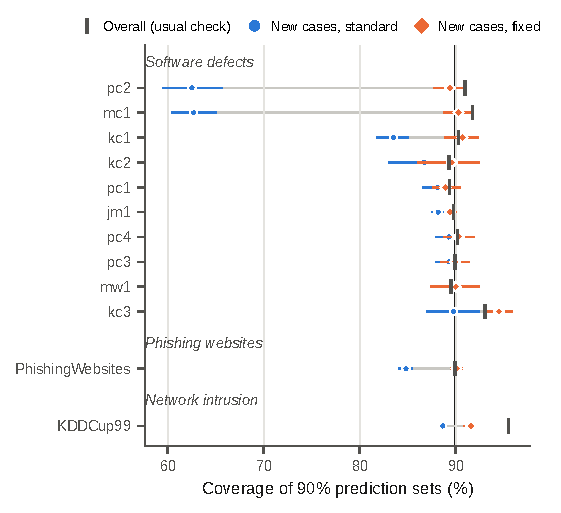
\includegraphics[width=0.62\textwidth]{figures/fig_cases.pdf}
\caption{In the three applications, the usual check reports about 90\% coverage while new cases are covered much less often, and separate calibration restores the target. Random forest, 90\% target, 10 random splits; error bars are 95\% bootstrap intervals of the mean over splits}\label{fig:cases}
\end{figure}

\begin{table}[!htbp]
\caption{Applications at a 90\% target (random forest; means over 10 random splits; LightGBM in Supplementary Table~\ref{S-tab:casesfull}). Seen: share of test rows with an exact training copy. $g^*$: predicted gap from the check (no model). Overall: coverage reported by the usual check. New, std / New, fix: coverage of new cases without and with separate calibration. Size: mean set size for new cases, standard and fixed}\label{tab:cases}
\centering\scriptsize
\setlength{\tabcolsep}{2.5pt}
\begin{tabular}{@{}lcrrrrrr@{}}
\toprule
Data & Model & Seen (\%) & $g^*$ (pp) & Overall & New, std & New, fix & Size std\,/\,fix\\
\midrule
\tabinput{tables/tab_cases_rf.tex}
\botrule
\end{tabular}
\end{table}

\subsection{Statistical analysis by hypothesis}\label{sec:res-hyp}

\paragraph{H1: the typical benchmark is not affected.} Repeated rows are common: \NNAnyDup{} of the \NNTotal{} benchmark data sets contain at least one, and in \NNDupGeThreeZero{} at least 30\% of rows belong to a group of identical rows. Exposure (Eq.~\ref{eq:exposure}) predicted the observed share of seen test rows almost exactly (mean absolute error \NExpMae{}). The planned test of a general shortfall was negative. The median new-case gap was between \NHOneGapMedianMin{} and \NHOneGapMedianMax{}\,pp across learner--score families, and no family was significant after Holm correction (smallest adjusted $p$ = \NHOneMinPHolm{}). Shortfalls were concentrated where many test rows are seen. Where at least 30\% are seen, \NXHiShareTwo{}\% of data set--learner pairs fell more than 2\,pp short and \NXHiShareFive{}\% more than 5\,pp. The worst gaps were \NHOneWorstGapCls{}\,pp (classification) and \NHOneWorstGapReg{}\,pp (regression).

\paragraph{H2: copies cause the shortfall.} Appending exact copies to the \NNdN{} duplicate-free data sets raised exposure as Eq.~(\ref{eq:exposure}) predicts, and the gap grew with it (Fig.~\ref{fig:inject}). For random forests in classification, the median gap went from \NInjClassificationRfZeroGap{}\,pp without copies to \NInjClassificationRfZeropFiveGap{}\,pp with half of the rows copied and \NInjClassificationRfOneGap{}\,pp with all rows copied. The regression figure with all rows copied was \NInjRegressionRfOneGap{}\,pp. LightGBM behaved similarly. Regularized linear models, which do not memorize rows, were barely affected (\NInjClassificationLogregOneGap{}\,pp). Separate calibration stayed at the target at every rate.

\begin{figure}[!htbp]
\centering
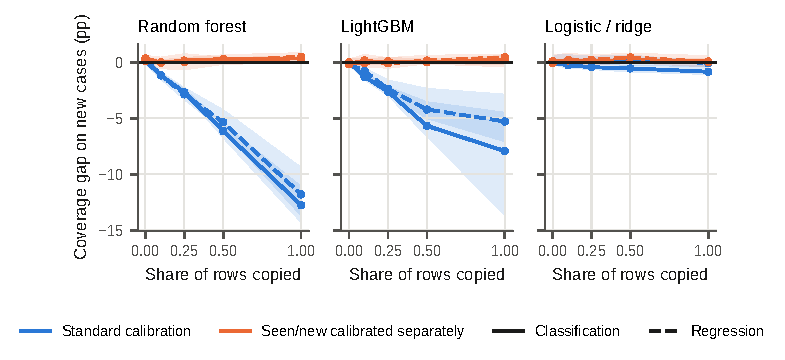
\includegraphics[width=\textwidth]{figures/fig_inject.pdf}
\caption{Copying rows on purpose creates the shortfall for flexible learners, in proportion to the share copied, while separate calibration stays on target. Median new-case gap over the \NNdN{} duplicate-free benchmark data sets; bands are 95\% bootstrap intervals of the median}\label{fig:inject}
\end{figure}

\paragraph{H3 and H4: the fix keeps its promise at little cost.} On the benchmarks with repeats, the median new-case gap of separate calibration ranged from \NHTwoMcpMedianRange{}\,pp, and the confidence interval of the median stayed above $-1$\,pp in \NHTwoNoninfAll{} learner--score combinations. Figure~\ref{fig:validity}a shows target against achieved coverage at three target levels. The overall coverage of standard calibration matches the target and its new-case coverage falls below it, while separate calibration matches the target for new cases. On the \NScpN{} fresh data sets (Fig.~\ref{fig:validity}b), the worst data set's gap with the fix was \NPrThreeRfMCPWorst{} (wave~1) and \NWTwoFixRfWorst{}\,pp (wave~2) for random forests. For LightGBM it was \NPrThreeLgbmMCPWorst{} and \NWTwoFixLgbmWorst{}\,pp, and for linear models \NPrThreeLogregMCPWorst{} and \NWTwoFixLogregWorst{}\,pp. Without the fix, the worst gaps were \NPrThreeRfSCPWorst{} and \NWTwoSCPRfWorst{}\,pp. The cost was small. On the benchmarks, sets for new cases grew by a median factor of \NHThreeNovelRatioRange{}, and on the wave-1 data by \NPrSizeMcp{}.

\begin{figure}[!htbp]
\centering
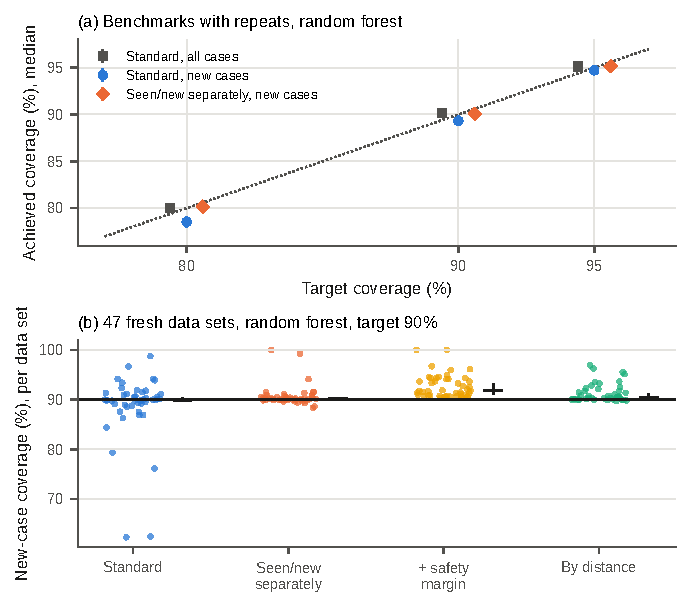
\includegraphics[width=\textwidth]{figures/fig_validity.pdf}
\caption{Target versus achieved coverage. (a) Benchmark data sets with repeats, random forest: standard calibration meets the target overall but not for new cases, while separate calibration meets it for new cases. Medians over data sets with 95\% bootstrap intervals. (b) The \NScpN{} fresh data sets at a 90\% target: new-case coverage per data set (dots) and medians with 95\% bootstrap intervals (black)}\label{fig:validity}
\end{figure}

\paragraph{H5--H7: the check on fresh data.}\label{sec:res-fresh} Figure~\ref{fig:screen} plots the predicted gap against the observed gap for all \NScpN{} fresh data sets.
\begin{itemize}
\item \emph{H5 (limit).} The predicted gap held as a limit. The random forest's gap stayed above $g^*-2$\,pp in \NPrRfAbove{}\% of wave-1 data sets (95\% CI \NPrRfAboveCi{}\%) and in \NWTwoRfAbove{}\% of wave-2 data sets (95\% CI \NWTwoRfAboveCi{}). The exception was \NWTwoViolNames{}.
\item \emph{H6 (ranking).} The predicted gap did \emph{not} rank the wave-1 data sets ($\rho$ = \NPrRfRho{}, Holm-adjusted $p$ = \NPrHolmPOne{}). Most of them have essentially no shortfall, so their ranks are decided by noise. It did rank the wave-2 data sets, which contain more real shortfalls ($\rho$ = \NWTwoRfRho{}, $p$ \NWTwoRfRhoP{}).
\item \emph{H7 (screening), the primary test of wave~2.} The combined flag caught all \NScTwoPos{} wave-2 data sets with a real shortfall (sensitivity \NScTwoSens{}, 95\% CI \NScTwoSensCi{}; Holm-adjusted $p$ = \NWTwoHolmWOne{}). Pooled over both waves, it caught \NScpHit{} of \NScpPos{} (95\% CI \NScpSensCi{}). Among the \NScpUnfl{} unflagged data sets, the worst gap for any learner was \NScpUnflWorst{}\,pp. The price is false alarms: specificity was \NScpSpec{}, but a false alarm only means applying a fix that costs almost nothing. The result depends little on where a ``real shortfall'' begins. With the flag rule unchanged, the check caught \NThrThreeHit{} shortfalls worse than $-3$\,pp and \NThrFiveHit{} worse than $-5$\,pp. With a looser threshold of $-1$\,pp it caught \NThrOneHit{}, missing three small shortfalls between $-1$ and $-2$\,pp (Supplementary Table~\ref{S-tab:threshold}).
\end{itemize}
The flagged shortfalls come from many domains. In wave~2 the random forest's gap was \NWTwodsSkinRf{}\,pp on skin segmentation, \NWTwodsDroidRf{}\,pp on Android malware permissions, \NWTwodsDiabRf{}\,pp on early diabetes risk and \NWTwodsVoteRf{}\,pp on voting records. LightGBM's gap on maternal health risk was \NWTwodsMatLgbm{}\,pp.

\begin{figure}[!htbp]
\centering
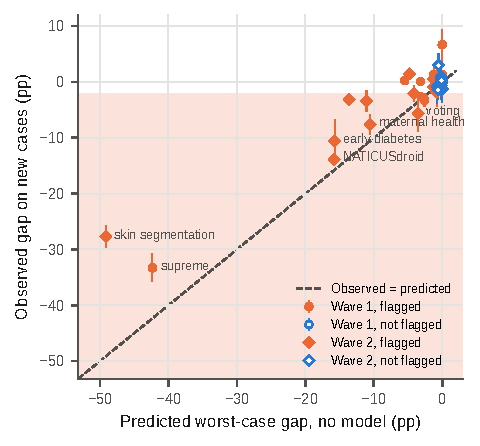
\includegraphics[width=0.62\textwidth]{figures/fig_screen.pdf}
\caption{On the \NScpN{} fresh data sets, every data set with a real shortfall (shaded, worse than $-2$\,pp) was flagged by the check before training. Observed gap: the worse of random forest and LightGBM, mean over 20 splits with a 95\% bootstrap interval. Filled markers: flagged; open markers: not flagged}\label{fig:screen}
\end{figure}

Label purity mattered in both directions. In black\_friday (\NPrBfPi{} of test rows seen), seattlecrime6 (\NPrScPi{}) and superconduct (\NPrCondPi{}), repeated rows almost never agree on the exact target. Exposure alone predicts gaps of \NPrBfGp{}, \NPrScGp{} and \NPrCondGp{}\,pp, while purity predicts none. The random forest's gaps were \NPrBfRfGap{}, \NPrScRfGap{} and \NPrCondRfGap{}\,pp. Over-coverage of new cases also has an explanation. On airlines, the predicted worst case was \NPrAirGs{}\,pp but the observed gap was \NPrAirRfGap{}\,pp. We had first attributed this to tied scores. The pre-specified tie-breaking test refuted that: with random tie-breaking, airlines' gap stayed at \NTbAirRand{}\,pp. Across the \NTbN{} highly exposed data sets, mean over-coverage fell only from \NTbOverScp{} to \NTbOverRand{}\,pp ($p$ = \NTbP{}). The data point instead to the mirror image of memorization. Seen airlines rows were covered only \NMirAirSeen{}\% of the time, because identical flight profiles carry conflicting delay labels. By Eq.~(\ref{eq:decomp}), new rows must then be over-covered (\NMirAirNew{}\%). Diabetes130US behaved the same way (seen \NMirDiaSeen{}\%, new \NMirDiaNew{}\%).

\paragraph{H8: the safety margin.} With separate calibration, \NPrFourRfMcp{}\% of wave-1 splits had new-case coverage below 87\% (random forest). With the safety margin this fell to \NPrFourRfPac{}\%; in wave~2 it fell from \NWTwoFixRfBad{}\% to \NWTwoPACMCPRfBad{}\%. Because most data sets had no unlucky splits at all, the planned wave-1 test was not significant after Holm correction ($p$ = \NPrHolmPFour{}). The margin enlarged sets by a factor of about \NPrSizePac{}.

\paragraph{H9: purity against exposure.} The advantage of purity over exposure alone for \emph{ranking} was not established on wave~1 (difference in $\rho$, 95\% CI \NPrRfDiffci{}). Its value lies in the screening decision, where it removes false alarms, as described above.

\paragraph{Is the variation just noise?} \emph{Post hoc.} Under exchangeability, the coverage of a split follows a known Beta--binomial law given the numbers of new calibration and test rows. We simulated it for every fresh split and compared the expected number of bad splits with the observed number (Supplementary Table~\ref{S-tab:noise}). For separate calibration with random forests, \NNoiseMCPRfObs{} bad splits were observed against \NNoiseMCPRfExp{} expected from pure noise (ratio \NNoiseMCPRfRatio{}, $p$ = \NNoiseMCPRfP{}). For standard calibration the ratio was \NNoiseSCPRfRatio{} ($p$ \NNoiseSCPRfP{}), so its shortfalls are real, not chance. LightGBM showed a small excess even with the fix (ratio \NNoiseMCPLgbmRatio{}, $p$ = \NNoiseMCPLgbmP{}), which we report but cannot explain with the data at hand.

\subsection{Qualitative analysis}\label{sec:res-qual}
\emph{Post hoc.} Supplementary Table~\ref{S-tab:examples} shows mc1 test modules chosen by a fixed rule, never by hand. The rule takes the first seen module, the first four new modules in data-set order, the first new defective module and the first new module that the fix misses. The standard threshold is very strict (\NExQStd{}) because most calibration rows are memorized copies with score zero. The new-case threshold of the fix is \NExQNew{}. Module 44 shows the typical repair: an empty set becomes a correct set. The failure cases are as instructive. The first new \emph{defective} module receives an empty set from both methods.


This points to a limitation that matters for defect triage. Only \NMcOneDefShare{}\% of mc1 modules are defective, so a coverage promise over all new modules says little about the defective ones. Over 10 splits, new defective modules (\NCcFixDefN{} in total) were never covered, by standard calibration (\NCcStdDefCov{}\%) or by the fix (\NCcFixDefCov{}\%). Calibrating by seen/new \emph{and} by class, which is label-conditional Mondrian calibration \citep{vovk2022}, covered them \NCcClsDefCov{}\% of the time. The cost is that most new modules then receive both labels (mean set size \NCcClsOkSize{} against \NCcFixOkSize{}): the model admits that it cannot tell. For rare but important classes, the fix should therefore be combined with class-wise calibration, which the tool offers as an option (\texttt{classwise=True}).

\subsection{Ablation study}\label{sec:res-ablation}
Table~\ref{tab:ablation} removes one part of the routine at a time. For the check, exposure alone flags \NAblExpoFlag{} of the \NAblNds{} fresh data sets and purity alone \NAblPureFlag{}. The combined rule flags \NAblCombFlag{} and catches all \NAblNpos{} real shortfalls. Purity alone misses one, black\_friday with a linear model, because a linear model cannot memorize rows and the shortfall there has a different cause. For the fix, removing separate calibration brings the shortfall back (Fig.~\ref{fig:validity}). Robustness checks against the most obvious alternative explanations come next.
\begin{itemize}
\item \emph{Target level.} The pattern holds at 80\%, 90\% and 95\% (Fig.~\ref{fig:validity}a).
\item \emph{Tied scores.} Random tie-breaking does not remove the effect (above).
\item \emph{Hyperparameters.} Making random forests less flexible lowered seen-row coverage, but the change in the gap was too small to detect at benchmark exposures (trend $p$ = \NCapClassificationRfP{}). We therefore rely on the learner comparison of Fig.~\ref{fig:inject} for the role of flexibility.
\item \emph{Near-copies.} Copies with noise of 0.1\% of a standard deviation are invisible to exact matching: the planted-leak test flagged \NLeakJitterRecall{}\% of them, but \NLeakRecall{}\% of \NLeakPlanted{} exact copies with no false positives. The shortfall persisted: the random forest's gap on truly new cases was \NNdClaZeropZeroSCP{}\,pp with exact copies and \NNdClaZeropZeroZeroOneSCP{}, \NNdClaZeropZeroOneSCP{} and \NNdClaZeropOneSCP{}\,pp with noise of 0.1\%, 1\% and 10\% of a standard deviation (Supplementary Fig.~\ref{S-fig:neardup}). Calibration by distance stayed at the target (\NNdClaZeropZeroDCP{}, \NNdClaZeropZeroZeroOneDCP{}, \NNdClaZeropZeroOneDCP{} and \NNdClaZeropOneDCP{}\,pp at the four noise levels) and matched an oracle that knows the true record identity.
\end{itemize}

\begin{table}[!htbp]
\caption{Ablation of the check on the \NAblNds{} fresh data sets, against the \NAblNpos{} data sets with a real shortfall (random forest or LightGBM gap below $-2$\,pp). Flag rules: exposure only ($\bar\pi\ge0.10$ or exposure-based gap below $-2$\,pp); purity only ($g^*<-2$\,pp); combined (either)}\label{tab:ablation}
\centering\small
\begin{tabular}{@{}lrrrr@{}}
\toprule
Flag rule & Flagged & Shortfalls caught & Correct no-flags & False alarms\\
\midrule
Exposure only & \NAblExpoFlag{} & \NAblExpoSens{} & \NAblExpoSpec{} & \NAblExpoFa{}\\
Purity only ($g^*$) & \NAblPureFlag{} & \NAblPureSens{} & \NAblPureSpec{} & \NAblPureFa{}\\
Combined (used) & \NAblCombFlag{} & \NAblCombSens{} & \NAblCombSpec{} & \NAblCombFa{}\\
\botrule
\end{tabular}
\end{table}


\subsection{Comparative analysis of remedies}\label{sec:res-remedies}
Table~\ref{tab:remedies} (and Supplementary Fig.~\ref{S-fig:remedies}) compare six options on the twelve application data sets, with the same splits and random forests (pre-specified, exploratory). What matters is which rows the calibration uses. Every remedy that calibrates on new rows brings new-case coverage to the target, and standard calibration does not. Removing repeats works about as well for new cases (\NRemDedupNewMed{}\% median), but it discards data: on mc1 the model is trained on \NRemMcOneTrainDedup{} instead of \NRemMcOneTrainFull{} modules. It also gives seen cases the sets calibrated for new ones, so they are over-covered (\NRemDedupSeenCov{}\%) with larger sets (\NRemDedupSeenSize{} against \NRemMCPSeenSize{} labels). A group split gives honest new-case coverage but says nothing about seen cases. On KDD Cup'99 it was infeasible in \NRemGscpKddFail{} splits, because a single group of identical connections exceeds the test part. Separate calibration keeps all data, works with any split and is valid for seen and new cases at once. In one small data set (mw1) fewer than nine seen calibration rows were available, so seen cases received the full set (Supplementary Fig.~\ref{S-fig:remedies}b).


\begin{table}[!htbp]
\caption{Remedies on the twelve application data sets (random forest, 90\% target, 10 random splits). New-case coverage: median and worst data set. Seen: coverage and mean set size for test rows with a training copy. Data used: median share of training rows kept}\label{tab:remedies}
\centering\footnotesize
\setlength{\tabcolsep}{3pt}
\begin{tabularx}{\textwidth}{@{}Xrrrrrr@{}}
\toprule
Method & \multicolumn{2}{c}{New-case coverage (\%)} & Empty sets & \multicolumn{2}{c}{Seen cases} & Data used\\
 & median & worst & new (\%) & cov. (\%) & size & (\%)\\
\midrule
\tabinput{tables/tab_remedies.tex}
\botrule
\end{tabularx}
\end{table}

\subsection{Computational complexity}\label{sec:res-cost}
The check hashes every row once and counts group sizes and label agreements. This is $O(N)$ hashing plus $O(N\log N)$ grouping, with memory linear in $N$. The fix adds one sort per group of calibration scores, $O(n_C\log n_C)$, the same order as standard split conformal prediction. Supplementary Table~\ref{S-tab:cost} gives measured times on the stated machine. The check took at most \NCostCheckMax{}\,s and \NCostCheckMemMax{}\,MB on 30,000 rows. Calibration with the fix took the same time as standard calibration (at most \NCostCalExactMax{} against \NCostCalStdMax{}\,s), because model inference dominates.


\subsection{Case study: the tool on NASA mc1}\label{sec:case}
A practitioner who runs \texttt{covercheck} on the mc1 file, with the defect label as target, sees the one-page report in Supplementary Fig.~\ref{S-fig:tool}. The check takes \NToolCheckS{}\,s and needs no model. It predicts a worst-case gap of \NToolGap{}\,pp, because \NToolPip{} of test modules will have a training copy with the same label, and it recommends the fix. The report then shows the problem directly: overall coverage of \NToolStdAll{}\%, but \NToolStdNew{}\% for new modules, \NToolStdEmpty{} of which receive an empty set. With the fix, new modules are covered \NToolFixNew{}\% of the time.

\emph{Real-world check of the tool.} \emph{Post hoc.} We ran the installed command-line tool, with its defaults, on \NTvN{} wave-2 data files downloaded fresh from the UCI repository. These were all wave-2 data sets with at most 30,000 rows, and the cached research pipeline was not used. The tool's exposure equalled the pipeline's to within $10^{\NTvExpDiffExp}$. Its verdicts agreed with the paper's rule on \NTvFlag{} of \NTvN{} files. Its new-case coverage agreed with the pipeline within two standard errors on \NTvFixTwose{} of \NTvN{} files (median difference \NTvMedFix{}\,pp), although preprocessing and seeds differ.


\subsection{Discussion}\label{sec:discussion}
\paragraph{What a practitioner should do.} First, run the check before training. In our data, a predicted gap no worse than $-2$\,pp together with fewer than 10\% seen test rows meant that nothing needed to change; this rule was written down before the fresh data were analysed. Second, if the data set is flagged, calibrate seen and new cases separately. Add the safety margin when fewer than a few hundred new calibration rows exist, and use calibration by distance when near-copies are plausible. Third, report new-case coverage next to the overall figure. In defect triage, intrusion detection or clinical screening, the reported coverage decides how many cases go to manual review. An empty set for a new defect-prone module is a silent failure that no overall figure reveals.

\paragraph{Limitations.} (i)~\emph{Exact matching only}: near-copies need calibration by distance (Supplementary Fig.~\ref{S-fig:neardup}), and a coarser match, such as rounding, is a modelling decision. (ii)~\emph{The predicted gap is a limit and a screen, not a forecast}: it did not rank the wave-1 data sets (H6), and it fails in both directions when Assumption~\ref{as:equal} fails, with a larger shortfall when slightly differing repeats are still easy (solar\_flare) and over-coverage when seen rows with conflicting labels are hard (airlines). (iii)~\emph{The typical benchmark is not affected} (H1), and varying flexibility within one learner was inconclusive; the problem is real but concentrated, which is why a check is useful. (iv)~\emph{Marginal over new cases, not per class}: a rare class (mc1 defects) needs class-wise calibration, at the cost of larger sets. (v)~\emph{Small calibration groups}: the safety-margin effect was not significant after correction (H8), and LightGBM showed a small excess of bad splits that we cannot explain. (vi)~\emph{No time order}: the NASA, intrusion and phishing data carry no time stamps, so we could not test deployments in which new releases arrive over time. (vii)~\emph{Few regression data sets in wave~2} (\NWTwoNCls{} of \NWTwoN{} are classification). (viii)~\emph{Same population}: distribution shift needs other tools, such as reweighting under covariate shift \citep{tibshirani2019} or bounds beyond exchangeability \citep{barber2023}. (ix)~\emph{Study conduct}: several analyses are post hoc and labelled as such, the plans were amended during the study (D1--D17), and the work was done with substantial AI assistance (Sect.~\ref{sec:framework}).

\section{Conclusions}\label{sec:conclusion}

This paper set out to answer a practical question: can a team trust the coverage of conformal prediction sets when it checks them on a random split of tabular data that contains repeated rows? The answer is that it often can, but not always, and that the cases where it cannot are predictable and repairable.

\paragraph{Strengths.} The study has four main strengths. First, the failure it describes is concrete and sometimes large. On NASA mc1 the usual check reported \NCsMcOneReported{}\% coverage while new modules were covered \NCsMcOneNew{}\% of the time, and \NToolStdEmpty{} of them received an empty set. Second, the check needs no model and runs in a fraction of a second. Its two quantities, the expected share of seen test rows and the share whose copies carry the same label, have exact closed forms. Third, the evidence was gathered under plans fixed in advance, on two fresh collections that played no part in developing the method. There the check flagged all \NScpPos{} data sets with a real shortfall, and with separate calibration new-case coverage never fell more than \NWTwoWorstFixAbs{} points below the target. Fourth, the routine is packaged as a tested open-source tool. It reproduced the research pipeline on \NTvN{} data files that we downloaded afresh.

\paragraph{Weaknesses.} The study also has clear limits. The predicted gap is a warning level and a limit, not a forecast: on the first fresh collection it did not rank data sets by the size of their shortfall. Its assumptions fail in both directions, giving larger shortfalls than predicted when slightly different repeats are still easy, and over-coverage when repeated rows with conflicting labels are hard. Exact matching misses near-copies, so calibration by distance is needed for them. A promise over all new cases does not protect a rare class, as the defective mc1 modules showed, and class-wise calibration is needed there at the cost of larger sets. All evidence comes from random splits of public data, not from a deployed system with records that arrive over time. Finally, several analyses were added after results were seen, and they are labelled as such.

\paragraph{Benefits to the field.} For practitioners in pattern recognition and machine learning, the routine turns a hidden failure into a visible and repairable one at almost no cost. It also gives authors of benchmark studies a simple reporting rule: state coverage on new cases next to the overall figure, and the share of seen test rows. Most standard benchmarks pass this check, which is reassuring. The data sets that fail it, in software defects, intrusion detection, phishing and several medical and security collections, are exactly those in which reported uncertainty may drive real decisions.

\paragraph{Future work.} Four directions follow directly.
\begin{enumerate}
\item Extend the check from exact to near-identical records, with a principled choice of matching resolution.
\item Combine the seen/new split with class-wise calibration for rare classes, and study the trade-off between coverage per class and set size.
\item Test the routine on time-ordered deployments, where future records are new by construction.
\item Build the check into common conformal-prediction libraries, so that new-case coverage is reported by default.
\end{enumerate}

\section*{CRediT authorship contribution statement}
\textbf{P. N. Bhargav Teja:} Conceptualization, Methodology, Software, Validation, Formal analysis, Investigation, Data curation, Visualization, Writing -- original draft.
\textbf{Rajay Vedaraj I. S.:} Conceptualization, Supervision, Project administration, Writing -- review \& editing.

\section*{Declaration of competing interest}
The authors declare that they have no known competing financial interests or personal relationships that could have appeared to influence the work reported in this paper.

\section*{Funding}
This research did not receive any specific grant from funding agencies in the public, commercial, or not-for-profit sectors.

\section*{Data availability}
All data sets are public. OpenML data sets are identified by their OpenML identifiers and UCI data sets by their UCI identifiers in the Supplementary Material, which also lists every excluded data set with its reason. The method is available as the open-source Python package \emph{covercheck}, and the complete research pipeline, with one command that reproduces every number, table and figure, is available in a version-controlled repository.

\section*{\raggedright Declaration of generative AI and AI-assisted technologies in the manuscript preparation process}
During the preparation of this work the authors used an AI system (a large language model with code-execution tools) to assist with the study design, the code, the experiments, the statistical analysis and the drafting of the manuscript. All numerical results were produced by executed code whose outputs are archived with the repository. After using this tool, the authors reviewed and edited the content as needed and take full responsibility for the content of the published article.


\bibliographystyle{elsarticle-num-names}
\bibliography{refs}

\end{document}
